% !TeX root = ../main.tex
% Add the above to each chapter to make compiling the PDF easier in some editors.

\chapter{Implementation}\label{chapter:implementation}

The following sections describe the implementation and explain the design decisions we made during development. 

\section{Technology Stack}

As our mobile platform, we have to decide between iOS and Android. While iOS has a more up-to-date operating system with 70\% of all of their mobile phones running iOS 13 and 23\% running iOS 12, Android has a much more significant market share with around 74\% compared to Apple's 25\% \cite{android1}\cite{android2}.

In terms of available development kits and libraries, both platforms provide plenty of choices. In the end, we choose Android, mainly because of their ease of deployment on devices for test scenarios. As for programming language, we opt for Kotlin instead of Java because of their intuitive syntax and compact and more readable codebase.

On the server-side of development, we select Node.js \cite{node} using Typescript combined with MongoDB's \cite{mongo} cloud storage solution, Atlas. Node.js provides a lot of flexibility with its vast ecosystem of third-party packages, and MongoDB, as a NoSQL database, easily stores and combines any type of data, allowing quick changes in the data model.

Our aggregation results can be fetched over the REST API or viewed directly in the MongoDB Atlas interface, given access privileges.

\section{REST API}
\label{sec:api}
We use a REST API based on the JSON data exchange format, and Table \ref{tab:rest} shows the endpoints.

\begin{table}[htbp]
\centering
  \begin{tabularx}{0.92\textwidth}{|l|X|}                                                                             \hline
        \multicolumn{1}{|c|}{\textbf{HTTP call}} & \multicolumn{1}{c|}{\textbf{Description}} \\ [0.5ex] 
        \hline
        POST /crowd HTTP/1.1 & Creates a new user and returns a password \\
        \hline
        POST /crowd/ping HTTP/1.1 & Updates the latest timestamp to current time \\
        \hline
        POST /aggregationRequest HTTP/1.1 & Initiates a aggregation request and forwards them to the device groups \\ 
        \hline
        POST /aggregationsteps HTTP/1.1 & Sends the intermediate step results of a group to the server for further processing  \\ 
        \hline
        POST /aggregationactivity HTTP/1.1 & Sends the intermediate activities results of a group to the server for further processing  \\ 
        \hline
        POST /aggregationlocation HTTP/1.1 & Sends the intermediate loaction results of a group to the server for further processing  \\ 
        \hline
        POST /aggregationpresence HTTP/1.1 & Sends the intermediate presence results of a group to the server for further processing  \\ 
        \hline
        GET /aggregationResult HTTP/1.1 & Retrieves a the results of an aggregation request \\ 
        \hline
  \end{tabularx}
  \caption{Description and usage of API endpoints shared by the Android application and the server.}
  \label{tab:rest}
\end{table}

The endpoints require authentication either as a requester or as a data collecting user. For the requester, we currently only create admin access by manually entering the username and password into the database. To register as users as participants in the crowd, they have to send their id and their public key, as depicted in Figure \ref{lst:registration}. The server provides the participants with a random password for future authentication for sending the result of their group.

\begin{lstlisting}[caption=Body of an HTTP request for creating a new user., label={lst:registration}]
    {
        "id": "35e78c9a6072b5e81ac2a5",
        "publicKey": "MIGfMA0GCSqGSIb3DQEBAQUAA4GNADCBiQKBgQCFEpvwtF76IsnmRxaPW7cDbzv4..."
    }
\end{lstlisting}

\section{Aggregation API}

To start an aggregation, Figure \ref{lst:request} shows the requesters have to send their \textit{username} and \textit{password} for authentication, the \textit{requestType} they want to aggregate and additional search options as \textit{request} depending on \textit{requestType} to the server. Example search options are visualized in the Listings \ref{lst:steps}, \ref{lst:activities}, \ref{lst:locations} and \ref{lst:presence}.

\begin{lstlisting}[caption=Body of an HTTP request for initiating a new aggregation with the server., label={lst:request}]
{
    "username": "admin",
    "password": password,
    "requestType": "steps" or "activities" or "location" or "presence",
    "request": see Listing 4.3, 4.4, 4.5 or 4.6
}
\end{lstlisting}

The following arguments used in the search options are:
\begin{itemize}
    \item \textit{start} and \textit{end} or \textit{date}: time of interest as an epoch integer
    \item \textit{lat} and \textit{lon}: coordinates of the point of interest as floating point integers
    \item \textit{radius}: distance to the point of interest in km as integer
    \item \textit{type}: type of activity as encoded in the Google Activity API \cite{detectedactivity}
    \item \textit{accuracy}: position after the comma to round for GPS accuracy as integer
    \item \textit{anonymity}: selected k for k-anonymity as integer
\end{itemize}

\begin{lstlisting}[caption=Search options of an HTTP request for steps data., label={lst:steps}]
{
    "date": 1582945200000,
    "lat": 35.535751,
    "lon": 139.629355,
    "radius": 50000
}
\end{lstlisting}

\begin{lstlisting}[caption=Search options of an HTTP request for activities data, label={lst:activities}]
{
    "type": 0,
    "start": 1582941600000,
    "end": 1582945200000,
    "lat": 35.535751,
    "lon": 139.629355,
    "radius": 50000
}
\end{lstlisting}

\begin{lstlisting}[caption=Search options of an HTTP request for location data, label={lst:locations}]
{
    "date": 1582945200000,
    "accuracy": 0,
    "anonymity": 2,
    "lat": 35.535751,
    "lon": 139.629355,
    "radius": 50000
}
\end{lstlisting}

\begin{lstlisting}[caption=Search options of an HTTP request for presence data, label={lst:presence}]
{
    "start": 1582941600000,
    "end": 1582945200000,
    "lat": 35.535751,
    "lon": 139.629355,
    "radius": 50000
}
\end{lstlisting}


When the server receives an aggregation request of the described form, it will send out a more detailed request to the device groups for data collection. The messages sent to the first mobile phones can be seen in Listing \ref{lst:aggregation}.

\begin{lstlisting}[caption=Body of an HTTP request starting a new aggregation with the devices., label={lst:aggregation}]
{
    "to": "35e78c9a6072b5e81ac2a5",
    "data": {
        "encryptionKey": null,
        "iv": null,
            "requestHeader": {
            "id": "618k1ndk71bvw1h",
                "start": 1582941600000,
                "end": 1582945200000,
                "type": "steps" or "activities" or "location" or "presence"
            },
            "requestOptions": {
                "groupNumber": 0,
                "numberOfGroups": 1,
                "from": "token",
                "group": []
            },
            "requestData": see Listing 4.3, 4.4, 4.5 or 4.6,
            "data": {
                "n": 0,
                "raw": []
        }
    }
}
\end{lstlisting}

After receiving and adding their data, the phones encrypt the \textit{data} JSON object and forward a similar message as Listing \ref{lst:aggregation} to the next device in the list. After reaching the last, they send the results back to the server. The messages to the server include the password generated on registration for authentication.

The implementation of the different JSON formats are flexible and can accommodate more aggregation types. The next sections will describe the features and the process of aggregation more in-depth from the Android device's and the server's point of view.

\section{Android Application}
As our target version of Android, we choose Android 10 (API level 29), which is currently the latest version of Android, and as a minimum version, we select Android KitKat (API level 19). The latest reports \cite{android3}\cite{android4} show that around 98\% are on Android KitKat or later. To collect mobility data, we leverage the power of Google Play Services. For persistent storage, we make use of the Room Persistence Library \cite{room}, as it provides an abstraction layer over SQLite and is commonly used in a lot of Android applications.

Because the platform relies on the generation of data from the crowd, the main features of the application are the collection of mobility data and providing the data on request. Figure \ref{fig:modules} describes the android application's architecture with its three main packages:

\begin{itemize}
    \item \textit{User Interfaces}: This package handles the start of the application and the presentation of the stored data.
    \item \textit{Background Services}: This starts all the processes in the background and manages all data collection and communications.
    \item \textit{Data Storage}: This part saves and fetches all the collected data stored in the Room database.
\end{itemize}

\begin{figure}[htpb]
  \centering
  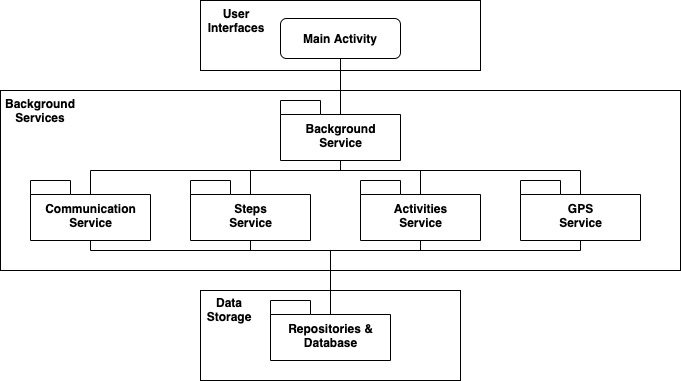
\includegraphics[width=0.8\textwidth]{figures/modules}
  \caption{Architecture with four decoupled main modules con- trolled by the \textit{Background Service}.} \label{fig:modules}
\end{figure}

On starting up, the application opens into the \textit{Main Activity}, where it asks the users for permission to access location services. On acceptance, the application starts the background services for data collection explained in the next section. It also serves the purpose of displaying stored data. We implement a screen for each type: steps, activities, and GPS. Using van Endern's Android application as a blueprint, we implement the same features to keep our application running behind the scenes. Because of background limitations Android introduced with Android Oreo, we create a non-dismissible notification and display it in the status bar and the notification center. It turns the application into a foreground application, bypassing the limitations set in the newer Android versions. To keep user interaction to a minimum, we enable the application to reopen when it crashes or is closed, and when we reboot it.

\subsection{Data Collection}
After the users successfully accept all permissions, the \textit{Main Activity} starts the \textit{Background Service}. The \textit{Background Service}, in turn, starts four tasks that have been shown in Figure \ref{fig:modules}. We loosely couple the four modules and separate them by data type or task at hand. We split the application into data collection and data aggregation. The aggregation process will be further explained in the next section. The data collection has three modules:
\begin{itemize}
    \item \textbf{Steps Module}: This module handles two classes, the \textit{Steps Service}, and the \textit{Steps Logger}. If the mobile phone has a pedometer, it registers the sensor to update the step count. The \textit{Steps Logger} receives steps from the sensor and stores it in the \textit{steps\_table} ever minute. Every step entry has an \textit{start} and \textit{end} timestamp and the number of steps taken in that time frame as \textit{steps}.
    \item \textbf{Activities Module}: This, similar to the \textit{Steps Service}, is composed of the \textit{ Activities Service} and the \textit{Activities Logger} classes. The \textit{ Activities Service} leverages Google's Activity Recognition API to identify the current activity of the mobile device. We are only interested in the main activities: still, walking, running, on a bicycle or in a vehicle. Therefore, for all possible activities, we register the transition type of entering or exiting the activity. Whenever we switch activities, the \textit{Activities Logger} writes the \textit{timestamp}, the \textit{type} and wether we \textit{enter}ed or not into the \textit{activities\_table}. Additionally, we store the exited activity into the \textit{activitiesDetailed\_table} with the \textit{start} and \textit{end} timestamp and the \textit{type}.
     \item \textbf{GPS Module}: This part of the application has the same structure as the other two described above. The \textit{GPS service} accesses Google's Fused Location Provider API to collect location data. The API itself uses the GPS sensor as well as the network sensors in the device to determine device location. We make the location sample rate dependent on the current activity because the positional changes between \textit{still} and \textit{on a bicycle}, for example, are very different. So we set the interval to 5 minutes for \textit{still}, 30 seconds for \textit{walking} and 15, 5 and once per second for \textit{running}, \textit{on a bicycle} and \textit{in a vehicle} respectively. Every once in a while, the \textit{GPS logger} receives batches of data from the API and saves them into the \textit{gps\_table} with their  \textit{timestamp}, \textit{lat}itude and \textit{lon}gtitude.
\end{itemize}

\subsection{Aggregation}
The last part of the background services is the communication module. It is in charge of passing on data from the server or devices to the next target using the push service specified in out design in Chapter \ref{chapter:design}.

\subsubsection{Push}
For our forwarding service, we select Pushy \cite{pushy} because of their free entry barrier and independence from big tech companies, as well as having implementations for both iOS and Android. Additionally, Pushy makes use of MQTT \cite{mqtt}, a light-weight messaging protocol that uses a small amount of bandwidth. We could also have used Firebase Cloud Messaging to forward messages, but giving Google more data to work is what we are trying to avoid.   Of course, the modular architecture of the app enables us to swap this method of communication for a peer-to-peer solution as soon as one proves applicable.

The communication service, communication receiver, and communication handler manage the complete communication infrastructure. After starting the application, the \textit{Background Service} creates the communication service that registers the device to the push service and receives a token as identification. Then it generates an asymmetric RSA key pair and registers itself to our platform with the Pushy token as \textit{id} and the \textit{publicKey} over the REST API. As a reply, the mobile phone receives a random password for future authentication purposes mentioned previously.

The communication receiver works as the entry point for push notifications from the push service and adds relevant data to the message. Upon receiving an aggregation request like in Listing \ref{lst:aggregation}, it checks for encryption and, if required, decrypts the data field. The application then aggregates data according to the \textit{type} sent in the \textit{requestHeader}:
\begin{itemize}
    \item \textbf{steps}: We add up the number of steps from the start and end of the specified day and add it to the list of raw values.
    \item \textbf{activities}: In this case, we sum up the time spent on the specified activity in the defined time frame and add that to the list of raw values.
    \item \textbf{location}: Here, we look for locations with the closest timestamp to the date specified in the header, but also inside a reasonable time, i.e., 10 minutes to cover the fact that still activities only logs the GPS data every 5 minutes. Then we spatially cloak the GPS coordinates and add it to the list of raw values as the hidden GPS position.
    \item \textbf{presence}: We just check all the GPS coordinates in the specified time frame, if they have been inside the range of the point of interest and add a 1 for if it has been and a 0 it has not.
\end{itemize}

After that, the communication handler takes the message and prepares it for the next participant in the \textit{group} array encoded in \textit{requestOptions}. If the device was the last in the list, it sends the results back to the server; otherwise, it uses the hybrid encryption scheme to encrypt data with the credentials of the subsequent device. So the current device generates a symmetric AES key and encrypts the \textit{data} and afterward does the same to the symmetric key using the public RSA key of the selected participant. Next, the communication handler forwards it over the push service, which in turn sends a push notification to the specified mobile phone. This repeats in each group until it chooses the last device.

\subsubsection{Spatial Cloaking}
Our version of interval cloaking creates rectangular areas by rounding digits. After receiving a request coordinates, the device select the closest entry to the specified \textit{date} and obfuscate it using the \textit{accuracy} parameter provided in the aggregation request. For example, the GPS coordinates \((48.262531, 11.668090)\) will be cloaked in the area with the coordinates \(\langle(48.26, 11.66),(48.27, 11.67)\rangle\), when using an accuracy of 2. We then use the haversine formula to calculate the midpoint of the two corner points as a representative for the cloaked space. 

\subsubsection{Bypassing inactive users in the aggregation chain}
In the case, that the aggregation is stuck because of any reason, for instance, a device does not have an internet connection, it is turned off, or the participant deleted the application, we have to be able to bypass the inactive mobile phone and select a new one.

With our selected push notification service, the mobile phones periodically ping the push notification server, signaling that they are online and active. Using this information, we only send aggregation requests to the participants that are marked online by the service, bypassing devices that have been offline and have not contacted it in a while. However, it could also be the case that the mobile phone is not available after the aggregation has already started.

So after the users forward their encrypted results to the following device, they start a sleeping thread that will skip the next device and select the one after that. The subsequent user that receives the message from the push service will aggregate the data as usual but will send a short confirmation message back to the preceding participant, which cancels the sleeping thread, signaling that aggregation was successful. We do not need to skip the device.

By avoiding offline devices and actively confirming that a fulfilled request, we can bypass inactive users and make the aggregation more efficient and reliable.

\section{Server}
For our server, we are using Node.js, on version 12.12.21 with the express \cite{express} middleware, a minimal web application framework. Our MongoDB Atlas database instance receives data over the database communication module. We can see the architecture in Figure \ref{fig:server}.

\begin{figure}[htpb]
  \centering
  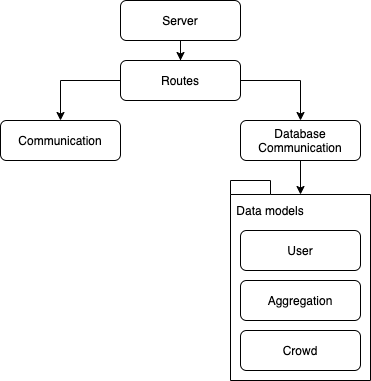
\includegraphics[width=0.5\textwidth]{figures/server}
  \caption{Modular architecture of the server seperated by communication type.} \label{fig:server}
\end{figure}

As our programming language, we select Typescript because of its versatility. As a superset of Javascript, it supports all Javascript libraries natively and allows for object-oriented programming paradigms. Also, it provides optional static typing and better code structure. However, to run the server, we transpile our Typescript code to Javascript code to run the webserver.

When we start the server, \textit{app.ts} registers the routes described in Table \ref{tab:rest} and connects the database object to the cloud storage instance. All calls to MongoDB are handled over that object, while the route handler manages calls to the endpoints.

\subsection{Registration}
Upon starting the application, it registers to the server using the JSON shown in Listing \ref{lst:registration} over the \textit{/crowd} route. To update the latest timestamp, we also have an obsolete route \textit{/crowd/ping}, which has been replaced with the ping our push notification service already provides. However, this route can be modified to ping the devices for their current status if another communication model is adapted.

\subsection{Aggregation}
We create one route to which the requesters can send their aggregation requests. After receiving a JSON in the mentioned form in the Listing \ref{lst:request} in route \textit{/aggregationRequest}, the server will get all the devices, ping them using the push service, select all the available participants and calculate the groups. Before assigning the groups, we use the Fisher-Yates shuffle to mix the order of the users. We calculate group sizes depending on a designated minimal length, so the aggregation has enough members in each group for anonymity purposes, but small enough to stay efficient. After all that, the server sends the aggregation request to all groups using the push service.

On request creation, the server creates a temporary aggregation object that stores the id, number of groups, and how many it already has received. We have four additional routes for the final aggregation, \textit{/aggregationsteps}, \textit{/aggregationactivity}, \textit{/aggregationlocation} and \textit{/aggregationpresence}. They each manage the POST requests from the Android devices and calculate data or ensure anonymity.

\subsection{Anonymity}
To achieve privacy with data as sensitive as whereabouts, we apply k-anonymity. For steps and activity, we do not see any immediate privacy issues and thus refrain from using k-anonymity as that would needlessly sacrifice the usability of the data without benefits. As opposed to location data, we merge the received spatially cloaked raw values and suppress all coordinates that do not fulfill our defined k. 

\section{Limitations}
Even with the proposed solutions, the architecture is still far from perfect. While the data should be confidential because of the state-of-the-art encryption, we still have to rely on a third party to deliver messages, making us dependent on their availability.

With van Endern's aggregation chain, the most vulnerable participants would be the first ones because the next user in line would always be able to see the raw data that the first users added. In our version, each group exposes the data of the first participant to the second. Unfortunately, homomorphic encryption is still expensive, and there are currently no available libraries for Android that implement it.

Our spatial cloaking algorithm is also imperfect. Interval cloaking has the disadvantage that the coordinates predetermine the cloaked areas. It might not group participants together, although they are close in proximity  because they are standing in different spatial regions.

Another issue that can lead to privacy issues is centralization. While the raw data itself is distributed, the control over aggregated data, its storage, and its collection is still under one central authority.